\documentclass[12pt]{report}
\usepackage[utf8]{inputenc}
\usepackage[czech]{babel}
\usepackage{geometry}
\usepackage{xcolor}
\usepackage{ragged2e}
\usepackage{hyperref}
\usepackage{graphicx} % Balíček pro práci s obrázky

\justifying
\setcounter{secnumdepth}{0}  % Zabránit číslování sekcí
\pagenumbering{gobble}

% Okraje stránky
\geometry{a4paper, left=30mm, right=30mm, top=25mm, bottom=25mm}

% Nastavení pro větší řádkování
\renewcommand{\baselinestretch}{1.5}

\begin{document}

\thispagestyle{empty}

% Ohraničení kolem textu

% Centrování obsahu
\begin{center}
    \textbf{\large Západočeská univerzita v Plzni}\\
    \textbf{\large Fakulta aplikovaných věd}\\
    \textbf{\large Katedra informatiky a výpočetní techniky}
    
    \vspace{2cm} % Vzdálenost mezi textem
    \vspace{1cm}
  
    \textbf{\Huge Bakalářská práce}
    
    \vspace{1cm}
 
    \textbf{\Huge Vytvoření Wordpress pluginu pro}\\
    \textbf{\Huge  vyhledávání předků pro Czech-American TV}
    
    \vfill
    \begin{tabbing}
    \hspace{8cm} \= \kill
    \textbf{Plzeň, 2025} \hspace{10cm} \textbf{Jan Čácha}
    \end{tabbing}
    
    \vspace{1cm}

\end{center}
\newpage  % Vložení nové stránky

\begin{center}
    \textbf{\Huge Originální zadání} % Nadpis
\end{center}

\vspace{1cm} % Vzdálenost mezi nadpisem a textem

% Zarovnání na levou stranu
\begin{flushleft}

    1. Prostudujte předchozí plugin s názvem \textbf{Genealogy} a související problematiku s vyhledáváním předků z jiného kontinentu.

    2. Analyzujte návrhy a informace od zástupce \textbf{Czech-American TV}.

    3. Navrhněte nový plugin.

    4. Plugin implementujte.

    5. Vytvořený plugin řádně otestujte.

    6. Kriticky zhodnoťte vytvořené řešení včetně vyhodnocení názorů zástupců \textbf{Czech-American TV} na vytvořené dílo.

\end{flushleft}
\newpage  % Vložení nové stránky

\begin{center}
    \textbf{\Huge Prohlášení} % Nadpis
\end{center}

\mbox{}
\vfill  % Vytlačení obsahu na dolní část stránky

\begin{minipage}{0.8\textwidth} % Šířka bloku
    \textbf{Prohlašuji, že jsem bakalářskou práci vypracoval(a) samostatně a výhradně s použitím citovaných pramenů.}

   \vspace{0.5cm} % Vzdálenost mezi podpisem a dalším textem

   V Plzni dne \underline{\hspace{5cm}} % Čára pro vlastnoruční podpis

    \vspace{0.5cm} % Vzdálenost mezi podpisem a dalším textem

    Podpis  \underline{\hspace{5cm}}  % Text pro jméno
\end{minipage}

\newpage 
\begin{center}
    \textbf{\Huge Abstract} % Nadpis
\end{center}

\vspace{1cm}

\begin{center}
    \textbf{\LARGE Creating a WordPress Plugin for Ancestry Search for Czech-American TV}
\end{center}

\vspace{1cm}  % Vzdálenost mezi titulkem a textem
This bachelor’s thesis focuses on the development of a WordPress plugin designed to facilitate ancestor searches for viewers of Czech-American TV. With the increasing interest in genealogy among the Czech diaspora, the need for effective tools to trace ancestry has become paramount. The project begins with an analysis of existing solutions, followed by gathering requirements from stakeholders, including representatives from Czech-American TV. Based on this analysis, a new plugin is proposed and implemented, incorporating user-friendly features for efficient search functionalities. The plugin is rigorously tested to ensure reliability and ease of use. This work contributes to enhancing the online experience for viewers interested in exploring their heritage, promoting a deeper connection with their roots.

\newpage
\begin{center}
    \textbf{\Huge Abstrakt} % Nadpis
\end{center}

\vspace{1cm}
Tato bakalářská práce se zaměřuje na vývoj WordPress pluginu, který má usnadnit vyhledávání předků pro diváky Czech-American TV. S rostoucím zájmem o genealogii mezi českou diasporou se potřeba efektivních nástrojů pro pátrání po předcích stala zásadní. Projekt začíná analýzou existujících řešení, následovanou shromážděním požadavků od zúčastněných stran, včetně zástupců Czech-American TV. Na základě této analýzy je navržen a implementován nový plugin, který zahrnuje uživatelsky přívětivé funkce pro efektivní vyhledávací možnosti. Plugin je důkladně testován, aby se zajistila jeho spolehlivost a jednoduchost použití. Tato práce přispívá k vylepšení online zážitku pro diváky, kteří se zajímají o zkoumání svého dědictví, a podporuje hlubší spojení s jejich kořeny.

\newpage  % Vložení nové stránky

\pagenumbering{gobble} % Skrytí číslování stránek před úvodem

\tableofcontents  % Vytvoření obsahu automaticky

\newpage

\pagenumbering{arabic} % Začátek číslování stránek od úvodu

\section{1. Úvod}
\vspace{1cm}
Czech-American TV je nezisková organizace, která se zaměřuje na podporu české kultury, historie a tradic mezi česko-americkou komunitou. Jednou z jejich klíčových aktivit je poskytování obsahu a nástrojů, které pomáhají lidem objevovat jejich rodinné kořeny a historii. V tomto kontextu vzniká bakalářská práce zaměřená na vytvoření pluginu pro systém WordPress, který bude součástí této platformy a usnadní genealogické hledání předků a historických souvislostí.

Motivace pro tento projekt vychází z rostoucího zájmu o genealogii a využívání digitálních nástrojů při hledání informací o předcích. Pro členy česko-americké komunity, kteří často čelí jazykovým bariérám a roztříštěným zdrojům informací, je důležité mít k dispozici centralizovaný a snadno použitelný nástroj. Tato bakalářská práce si klade za cíl vytvořit řešení, které nejenže poskytne technické možnosti vyhledávání, ale také obohatí uživatelský zážitek prostřednictvím moderních interaktivních prvků.

Navrhovaný plugin bude zahrnovat následující klíčové funkce:

\begin{enumerate}
    \item Interaktivní seznam měst s možností vyhledávání a filtrování podle regionu a historického období.
    \item Genealogickou mapu umožňující vizualizaci geografického rozložení jmen a měst.
    \item Rozšíření o filtrování podle pohlaví a regionu v sekci \textit{Changing Name}.
    \item Sekci pro překlady, která umožní uživatelům snadno převádět texty mezi angličtinou a češtinou.
\end{enumerate}

Práce je strukturována následovně:

V \textbf{kapitole 2} se zaměřujeme na analýzu stávajících řešení a jejich omezení. \textbf{Kapitola 3} popisuje návrh a architekturu pluginu, včetně technologií a metod použitých při jeho vývoji. \textbf{Kapitola 4} obsahuje implementační část, kde je detailně popsán průběh tvorby jednotlivých funkcionalit pluginu. \textbf{Kapitola 5} se zabývá testováním a evaluací vytvořeného řešení. Závěrem v \textbf{kapitole 6} shrnujeme dosažené výsledky a navrhujeme možnosti dalšího rozvoje.


\newpage
\section{2. Analytická část}
\vspace{1.cm}
\section{2. Analytická část}
\vspace{1.cm}
\subsection{2.1. Genealogie a její význam}
Genealogie, tedy studium rodokmenů a rodinné historie, má hluboký význam nejen pro historiky, ale i pro jednotlivce, kteří hledají své kořeny a snaží se porozumět svému původu. Na platformě Czech-American TV je patrný rostoucí zájem o propojení mezi Českou a americkou historií. Tento projekt si klade za cíl vytvořit nástroj, který usnadní uživatelům vyhledávání jejich předků a pochopení jejich historických souvislostí. Interaktivní nástroj umožní filtrování dat, vizualizaci informací na mapě a možnost překladu mezi češtinou a angličtinou.

\subsection{2.2. Technologický základ projektu}
Projekt bude realizován jako plugin pro redakční systém WordPress. Ten byl zvolen z následujících důvodů:
\begin{itemize}
\item \textbf{Rozšířenost a podpora}: WordPress je populární platforma s širokou komunitou a dostupnou dokumentací, což usnadňuje řešení technických problémů a integraci nových funkcí.
\item \textbf{Jednoduchost implementace}: WordPress poskytuje strukturu, která umožňuje rychlý vývoj a nasazení pluginů.
\item \textbf{Kompatibilita s existujícími systémy}: Platforma Czech-American TV již WordPress využívá, což zajišťuje bezproblémovou integraci a rozšíření stávajících funkcionalit.
\item \textbf{Flexibilita}: WordPress je otevřená platforma, která umožňuje výraznou míru přizpůsobení.
\end{itemize}



\subsection{2.3. Machine Learning v genealogii}
Strojové učení představuje moderní technologii, která má v genealogii významný potenciál. Umožňuje analyzovat rozsáhlé soubory historických dat, identifikovat vzory a navrhovat rodinné vztahy na základě pravděpodobnosti. Implementace technik strojového učení v rámci genealogického výzkumu může výrazně zlepšit přesnost a rychlost vyhledávání informací, zejména v případech, kdy se jedná o historicky změněná jména, neúplné záznamy nebo geograficky vzdálené zdroje dat.

Cílem je vytvořit nástroj, který bude využívat strojové učení k posílení genealogického výzkumu. Součástí tohoto projektu je implementace algoritmu Word2Vec, který pomůže při vyhledávání jmen a jejich variant. Tím se zlepší přístup uživatelů k historickým datům, která mohou být obtížně dostupná z důvodu jazykových a kulturních odlišností.

\subsubsection{Word2Vec a jeho využití v genealogii}
Algoritmus Word2Vec je jednou z klíčových metod pro zpracování textových dat v oblasti strojového učení. Tento algoritmus převádí slova do matematických vektorů, což umožňuje měřit podobnosti mezi nimi pomocí geometrických operací. Word2Vec využívá dva hlavní modely:
\begin{itemize}
    \item Skip-Gram: Modeluje pravděpodobnost okolních slov na základě aktuálního slova.
    \item CBOW (Continuous Bag of Words): Modeluje pravděpodobnost aktuálního slova na základě okolních slov.
\end{itemize}

Použití Word2Vec v genealogii má několik praktických přínosů:
\begin{itemize}
    \item \textbf{Identifikace podobných jmen}: Algoritmus dokáže najít historické varianty jmen (například Novák a Nowak) na základě jejich kontextu v textových záznamech.
    \item \textbf{Klasifikace původu jmen}: Vektorová reprezentace umožňuje klasifikaci jmen podle geografického původu či historického významu.
\end{itemize}

\subsubsection{Matematický model Word2Vec}
Algoritmus Word2Vec převádí slova na vektory \( \vec{w} \) v n-rozměrném prostoru. Pro měření podobnosti mezi dvěma slovy \( w_1 \) a \( w_2 \) se používá kosinová podobnost:

\begin{equation}
\mathrm{cosine\_similarity}(\vec{w}_1, \vec{w}_2) = \frac{\vec{w}_1 \cdot \vec{w}_2}{\|\vec{w}_1\| \cdot \|\vec{w}_2\|}
\end{equation}


Kde \( \vec{w}_1 \cdot \vec{w}_2 \) je skalární součin a \( \|\vec{w}_1\|, \|\vec{w}_2\| \) jsou velikosti vektorů. Kosinová podobnost nabývá hodnot od -1 do 1, přičemž hodnoty blízké 1 znamenají vysokou podobnost mezi slovy.

\subsubsection{Praktická implementace Word2Vec}
Pro potřeby genealogie bude Word2Vec využit k:
\begin{itemize}
    \item Rozpoznávání příbuzných jmen: Algoritmus bude schopen identifikovat jména se společným kořenem nebo jména, která prošla historickými změnami (například změny pravopisu při migraci).
    \item Zlepšení vyhledávacích funkcí: Uživatelé budou schopni zadávat klíčová slova a získávat odpovídající výsledky, které zahrnují i historicky odvozené nebo překládané varianty.
\end{itemize}

\subsection{2.4. Zpracování RTF souboru}
Jedním z klíčových kroků bylo zpracování velkého RTF souboru obsahujícího genealogická data. Soubor měl velikost přibližně 10 MB a obsahoval tisíce záznamů ve formátu podobném tabulkovému uspořádání. Struktura dat zahrnovala informace o slovech a jejich překladů Českého jazyka do Anglického jazyka. Pro jejich zpracování byl vyvinut skript v Pythonu, který data převedl do strukturované podoby a importoval do relační databáze. Tento krok zajišťuje rychlé vyhledávání a filtrování dat podle různých kritérií.

\subsubsection{Databáze a její struktura}
Data jsou uložena v relační databázi, která je navržena tak, aby umožňovala rychlé filtrování a třídění informací o městech, jménech a překladech.

\begin{figure}[h!]
    \centering
    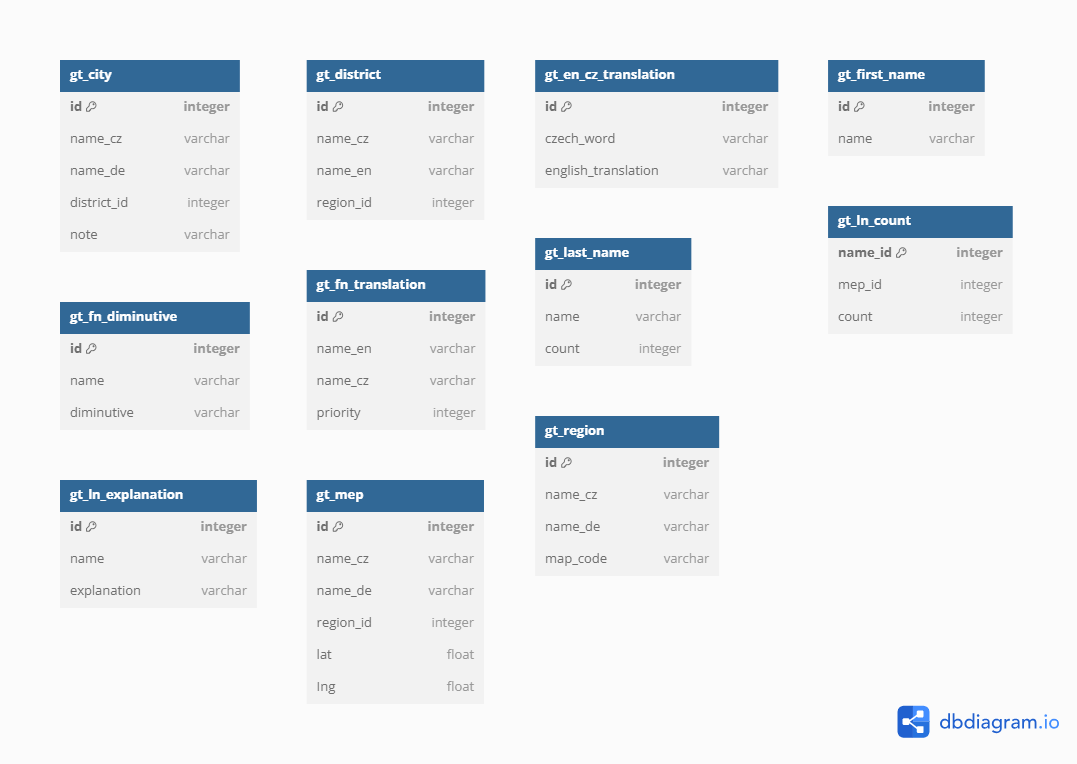
\includegraphics[width=\textwidth]{datagram.png}
    \caption{Tabulky databáze}
    \label{fig:obrazek}
\end{figure}


\subsection{2.5. Interaktivní seznamy a filtry}

\subsubsection{Filtr pro města a období}
Uživatelé budou moci filtrovat města podle historického období či regionu. To umožní například vyhledat města, kde jejich předci žili v určitém časovém období. K tomu využijeme JavaScript a AJAX pro dynamické načítání dat, což zaručí rychlou odezvu systému.

\subsubsection{Filtrovaní jmen podle původu a genderu}
Další interaktivní funkcí bude možnost filtrování jmen podle genderu a původu. To uživatelům umožní zaměřit se na konkrétní skupiny jmen, což zlepší přesnost a efektivitu vyhledávání.

\subsection{2.6. Vizualizace a překladové funkce}

\subsubsection{Genealogická mapa}
Pro zlepšení uživatelské zkušenosti bude vytvořena interaktivní mapa, kde budou vizualizována města spojená s předky uživatele. Tato mapa bude implementována pomocí nástroje Leaflet, který umožňuje jednoduchou a flexibilní práci s geografickými daty. Uživatelé budou moci kliknout na město na mapě a získat další informace o obyvatelích či historických událostech.

\subsubsection{Překladové funkce}
Pro zajištění lepší dostupnosti informací pro široké publikum bude implementována překladová sekce, která umožní uživatelům překládat genealogická data mezi češtinou a angličtinou. Překlad bude realizován pomocí API nástroje Google Translate, což zjednoduší proces a zajistí spolehlivé překlady.

\subsection{2.7. Shrnutí}
Analýza existujících dat a technologií ukázala, že kombinace WordPressu a moderních metod strojového učení, jako je Word2Vec, poskytuje robustní základ pro vytvoření efektivního genealogického nástroje. Důležitou roli hraje kvalitní zpracování vstupních dat, které umožní uživatelům rychlé a intuitivní vyhledávání v rozsáhlých genealogických databázích.












\end{document}
